\subsection{Einlesen der Konfigurationsdateien} \label{einlesen_konfigurationsdateien}
\paragraph{Klassenstruktur}
Im Backend wird die Klassenstruktur der \ac{gui} nachgebildet. Es gibt eine \lstinline{Page}, eine \lstinline{Measurement} und eine \lstinline{Sensor} Klasse. Eine \lstinline{Measurement} Instanz kann mehrere \lstinline{Sensor} Instanzen enthalten, da manche \lstinline{Measurements} zur Berechnung (z.B. der Wärmerückgewinnungsgrad) mehrere Messwerte benötigen. Die \lstinline{Page} Instanzen speichern die jeweiligen \lstinline{Measurement} Instanzen, die auf dieser Seite angezeigt werden sollen. Die \lstinline{Page} Instanzen existieren, damit der ausgelesene Parameter an der richtigen Stelle auf der \acs{gui} verändert werden kann. Es gibt nämlich gleich viele \lstinline{Page} Instanzen wie \lstinline{PageFrame} Instanzen (vgl. Kapitel \ref{tkintercode}) und gleich viele \lstinline{Measurement} Instanzen wie \lstinline{MeasurementFrame} Instanzen. (siehe Abb.~\ref{fig:uml_backend}).
\begin{figure}[ht]
	\centering
	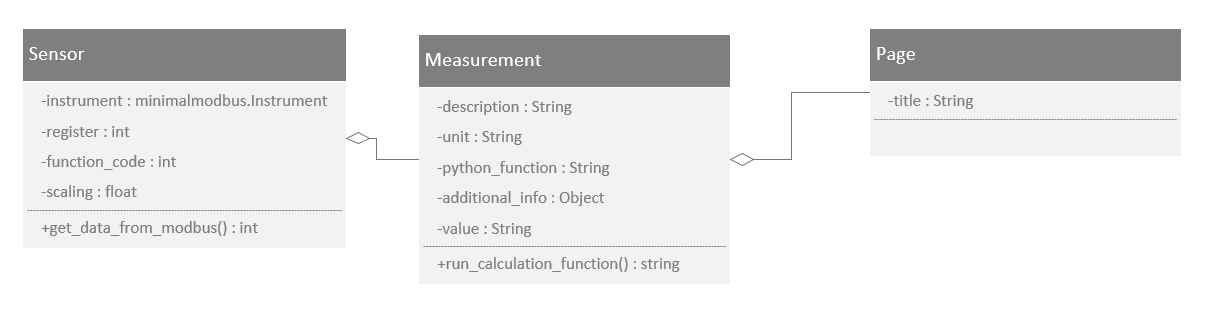
\includegraphics[width=1.0\linewidth]{Bilder/UML_Backend}
	\caption{UML Diagramm Backend}
	\label{fig:uml_backend}
\end{figure}

Die \lstinline{Page}, \lstinline{Measurement} und \lstinline{Sensor} Instanzen werden beim Einlesen der \acs{json} Konfigurationsdateien aufgrund der Objekte im \enquote{pages}  Array (vgl. Kapitel \ref{json_config_files}) erstellt und in Listen gespeichert. \newline
Zum Einlesen werden drei Funktionen implementiert:
\begin{itemize}
	\item \textbf{\lstinline{load_config()}:} Diese Funktion lädt die gesamte Haupt-Konfigurationsdatei ein. Es werden die angeschlossenen Geräte ermittelt und die \lstinline{Page}, \lstinline{Measurement} und \lstinline{Sensor} Instanzen erstellt. Dafür kommen die beiden folgenden Hilfsfunktionen zum Einsatz.
    \begin{itemize}
		\item \textbf{\lstinline{get_sensor_unit()}:} Liest die Sensor-Konfigurationsdateien ein. Dadurch können den Messwerten die richtigen Maßeinheiten zugewiesen werden.
		\item \textbf{\lstinline{get_sensor_data()}:} Liest aus der Geräte-Konfigurationsdatei am angegebenen Port die Parameter aus und liefert diese Parameter als \acs{json} Objekt zurück. Sie liest das Register, den \gls{modbus} Function Code und die Skalierung aus. Die Skalierung wird anhand der Maßeinheit aus der Sensor-Konfigurationsdatei ausgewählt.
	\end{itemize}
\end{itemize}

\paragraph{Einlesen und Erstellen der Instanzen}
Einlesen kann man ein \acs{json} Attribut mit folgender Syntax. Im folgenden Beispiel wird aus der Instanz namens \lstinline{page} das Attribut \enquote{title} gesucht und zurückgeliefert.
\begin{pythoncode}
title = page["title"]
\end{pythoncode}

Im folgenden Code werden die \lstinline{Measurement} Instanzen erstellt, indem die anzuzeigenden Messwerte aus dem \enquote{sources} Array iteriert werden. Anhand der Informationen der Objekte im \enquote{sources} Array werden dann die entsprechenden Geräte im \enquote{devices} Array herausgesucht. Es werden weitere Parameter aus der Haupt-Konfigurationsdatei ausgelesen, die zu dem entsprechenden Messwert gehören (z.B. die Bezeichnung oder die Einheit). Anschließend werden die \lstinline{Sensor} Instanzen erstellt und einer Liste beigefügt, da manche Measurements (z.B. die Rückwärmzahl) mehrere Messwerte benötigen. Diese Liste, sowie die vorher ausgelesenen Parameter werden beim Erstellen der \lstinline{Measurement} Instanzen dem Konstruktor übergeben und darin in Instanzvariablen gespeichert.
\begin{pythoncode}
page_measurements = []
for measurements in page["sources"]:
	measurements_sensors = []
	#[Auslesen weiterer Parameter der Haupt-Konfigurationsdatei (description, unit, python_function,additional_info)]
	#[Erstellen der Sensor Instanzen (Siehe nächster Codeblock)]
	page_measurements.append(Measurement(description=description, unit=unit, sensors=measurements_sensors, python_function=python_function, additional_info=additional_info))
\end{pythoncode}

Im folgenden Code wird für jeden Port (an jedem Port ist ein \lstinline{Sensor} angeschlossen) eines Geräts eine \lstinline{Sensor} Instanz erstellt. Alle \lstinline{Sensor} Instanzen werden der \lstinline{page_sensors} Liste beigefügt. Dafür gibt es im \enquote{sources} Array die einzelnen Ports. Das sind Wertepaare, die jeweils aus Gerät und \lstinline{Sensor} bestehen (vgl. Kapitel \ref{json_config_files}). Mit diesen beiden Werten kann dann das entsprechende Gerät im \enquote{devices} Array gefunden werden und darin der entsprechende Port im \enquote{sensors} Array. Mit der \lstinline{get_sensor_unit()} Funktion wird die Einheit erhalten und mit der \lstinline{get_sensor_data()} Funktion weitere Sensordaten. Diese werden beim Erstellen der \lstinline{Sensor} Instanz dem Konstruktor übergeben.
\begin{pythoncode}
port_counter = 0
for port in port_arr:
	device_id = list(port.keys())[port_counter] # example: QBM1
	port_id = port[device_id]  # example: AI1
	port_counter += 1
	
	for device in config_full_data[0]["devices"]:
		if device["id"] == device_id:
			#[Aufruf der get_sensor_unit Funktion]
			#[Auslesen der Geräteparameter in der Haupt-Konfigurationsdatei (baud_rate, mbaddress etc.)]
			#[Aufruf der get_sensor_data Funktion]
			measurements_sensors.append(Sensor(baud_rate=device["baud_rate"], ..., register=register, zero_based=device["zero_based"]))
\end{pythoncode}

Die \lstinline{Measurement} Instanzen sind nach dem Erstellen alle in einer Liste gespeichert. Zum Schluss werden \lstinline{Page} Instanzen erstellt. Die \lstinline{Measurement} Liste wird so aufgeteilt, dass maximal 5 Measurements auf einer Seite sind. Anhand dieser \lstinline{Page}- und \lstinline{Measurement} Instanzen wird beim Erstellen der \acs{gui} die Anzahl an Seiten übernommen, der Seitentitel und die Beschreibungen der Messwerte gesetzt (siehe Kapitel \ref{gui_design}). 
\begin{pythoncode}
counter = 0
last_slice = 0
for measurement in page_measurements:
	counter += 1
	if ((counter % 5) == 0) or (counter == len(page_measurements)):
		all_pages.append(Page(title=title, measurements=page_measurements[last_slice:counter]))
		last_slice = counter
\end{pythoncode}

%\pythonfile[firstline=125, lastline=197]{Code/modbus.py}

Im Konstruktor der \lstinline{Page}, \lstinline{Measurement} und \lstinline{Sensor} Klasse werden die ausgelesenen Variablen in Instanzvariablen gespeichert.